\documentclass[12pt,letterpaper]{article}
\usepackage[utf8]{inputenc}
\usepackage{amsmath}
\usepackage{amsfonts}
\usepackage{amssymb}
\usepackage{graphicx}
\usepackage{float} 
\usepackage{fontspec}
\usepackage{xeCJK} 
\setCJKmainfont{SimSun}
\usepackage[left=1.00in, right=1.00in, top=1.00in, bottom=1.00in]{geometry}
\author{Joseph  Chen}
\title{SVM summary}
\date{\today}

\begin{document}
\maketitle

\section{Motivation}
  \begin{figure}[H]
	\centering
	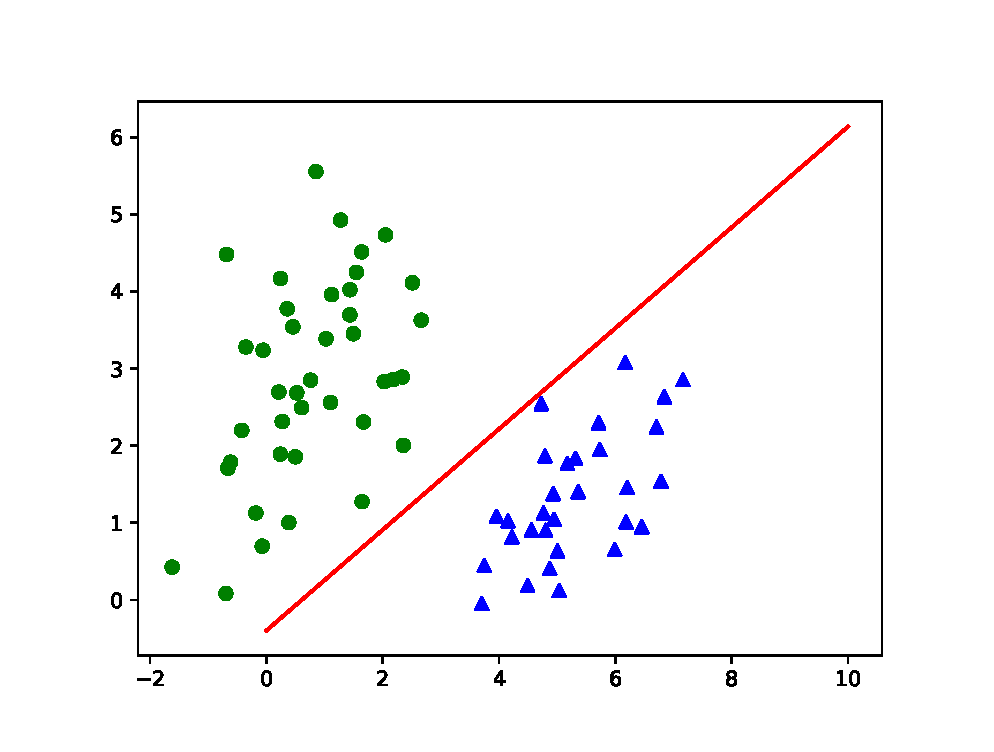
\includegraphics[width=0.6\textwidth, height=0.3\textheight]{linear_sp1}
	\caption{感知机训练得到的一个线性分类器}
  \end{figure}
假设两类模式线性可分, 如上图所示,绿色样本标记为正样本$+1$,蓝色样本作为负样本标记为$-1$. 用感知机的方法得到的一个线性分类器$y= w^Tx+b$, 给定一个新的样本$x$,决策过程
\[
	\text{if }w^Tx + b > 0 , \hat{y} = 1;\text{else } \hat{y} = -1
\]
这个分类器能用,然而不够鲁棒(Robust),也就是容易对噪声敏感(上图中分界面十分靠近蓝色).
SVM的想法就是在能够线性可分的条件下,尽可能增大到两类模式样本边界的距离,这样鲁棒性得到提升,
示意图如下
  \begin{figure}[H]
  	\centering
  	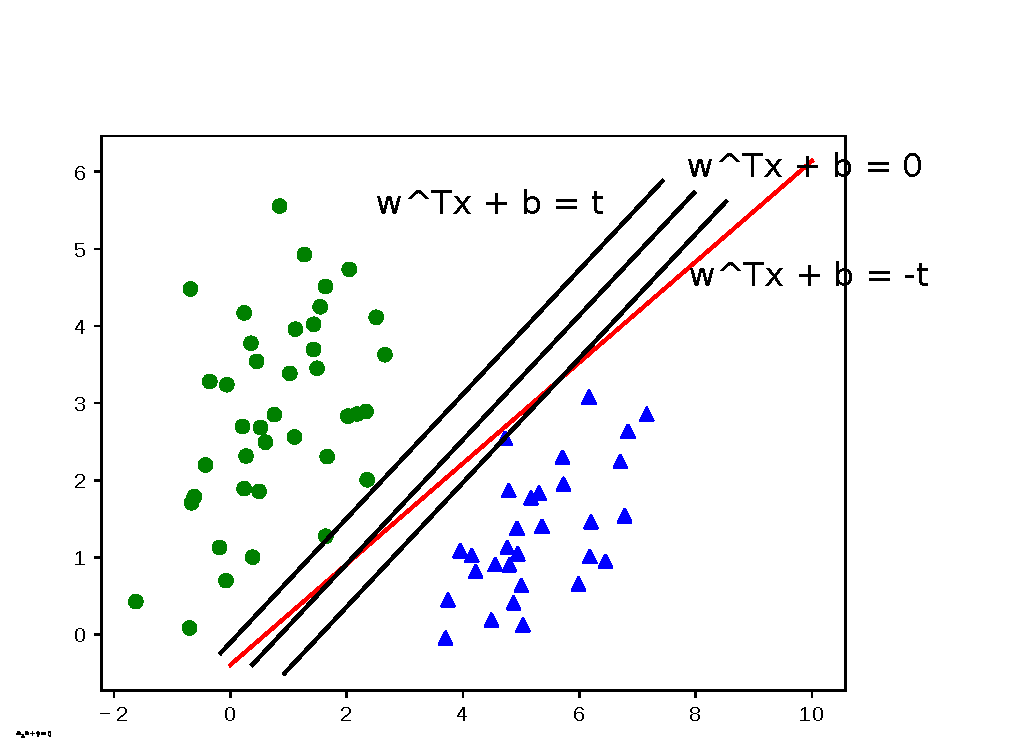
\includegraphics[width=0.6\textwidth, height=0.3\textheight]{linear_sp2}
  	\caption{margin}
  \end{figure}
  给定一个训练好的线性分类器$y=w^Tx+b$,对于正样本我们总有
  \[
	  w^Tx+b \geq  t > 0
  \]
 负样本
 \[
	 w^Tx + b \leq  -t < 0
 \]
 对所有样本(总数为$N$)分类正确,则
 \[
	 y^{(i)}(w^Tx^{(i)}+b) \geq t > 0 , i = 1,2,...,N
 \]
 我们想要做的是找到一个$w$和$b$,既能够将两类模式完全分开,又能尽可能最大化分界面$w^Tx+b=0$到两边的最小距离, 那么分界面当然选在两个边界的中间是最好的,
 最小距离的度量(求两条平行线的距离)
 \[
	 d = \frac{t}{||w||_2}
 \]
 所以整个问题变成了这个优化问题
 \[
    \begin{split} 
	 \max_{w,b}\quad  & \frac{t}{||w||_2} \\
	 \text{subject to } &  y^{(i)}(w^Tx^{(i)}+b) \geq t > 0 , i = 1,2,...,N 
	 \end{split} 
 \]
由于目标函数不是凸函数且多了$t$,不利于优化问题求解, 继续改进.
我们可以对$w$和$b$进行缩放(这样子做分界面的方程并没有改变),使得问题等价于
\[
    \begin{split} 
    \max_{w,b}\quad  & \frac{1}{||w||_2} \\
    \text{subject to } &  y^{(i)}(w^Tx^{(i)}+b) \geq 1 , i = 1,2,...,N 
    \end{split} 	
\]
 进一步地(因为$\frac{1}{||w||_2}$是非凸函数,继续变形), 最大化$\frac{1}{||w||_2}$就等价于最小化$\frac{1}{2}||w||_2^2$
 所以就得到了SVM问题的原始形式
 \[
    \begin{split} 
    \min_{w,b}\quad  & \frac{1}{2}{||w||_2^2} \\
    \text{subject to } &  y^{(i)}(w^Tx^{(i)}+b) \geq 1 , i = 1,2,...,N 
    \end{split} 	 
 \]
 这个问题形式是二次型,直接用凸优化就可以求解QP问题了, 举个例子(python跑的结果)
 \begin{figure}[H]
 	\centering
 	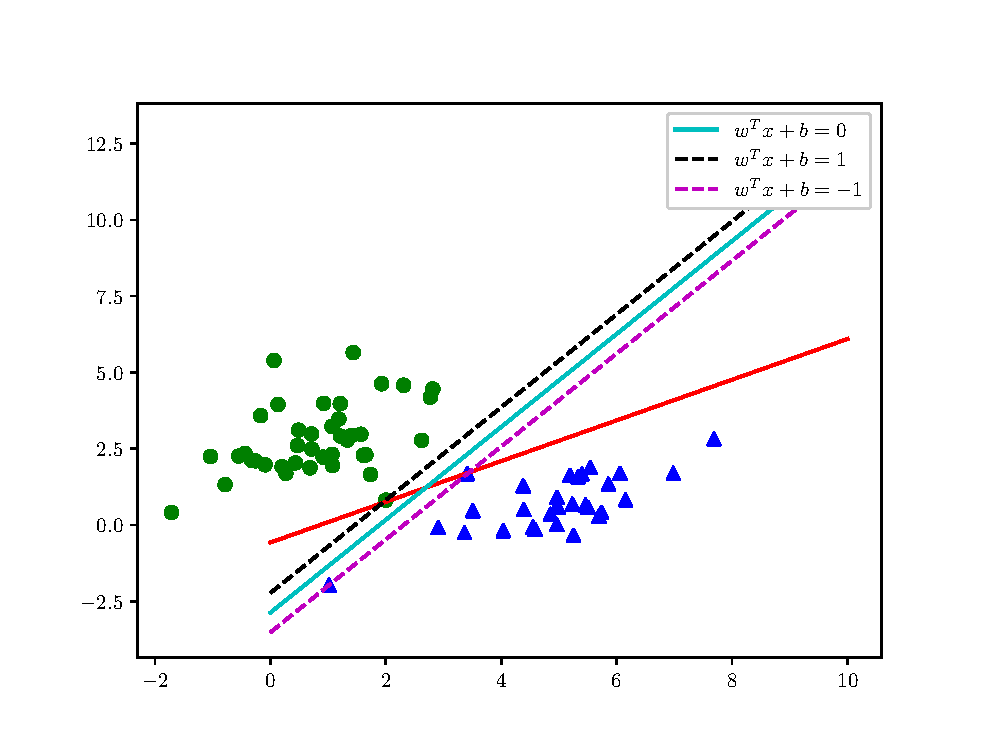
\includegraphics[width=0.6\textwidth, height=0.3\textheight] {svm_p}
 \end{figure}
红色曲线是由感知机训练得到的一个分类器, 紫色是直接解SVM原始问题得到的分类器,显然紫色的比红色的要好. 这里是用凸优化的工具直接求解得到参数, 后面之所以要用对偶是为了降低算法复杂度,用SMO算法也是为了加快速度,  用核方法是为了将低维度线性不可分的转到高维度线性可分.加上松弛是为了应付噪声, 原问题要求所有的样本点分类正确,所有有如下的约束
\[
   y^{(i)}(w^Tx^{(i)}+b) \geq 1 , i = 1,2,...,N
\] 
如果我们允许有个别点可以被忽略错误,比如正样本点越过分界面跑到了负样本那边, 
那么只需要添加辅助变量$\xi \geq 0$
\[
  y^{(i)}(w^Tx^{(i)}+b) \geq 1 - \xi_i, i = 1,2,...,N	
\]
道理很简单, 以正样本为例,如果出现正样本(图中绿色)跑到负样本方(蓝色区域), 
那么我们依然可以找到一个$t$(可正可负)使得所有正样本都满足
\[
   y^{(i)}(w^Tx^{(i)}+b) \geq t
\]
这里让$t= 1- \xi$既可,为了不使$\xi$过大(大了之后分类容忍距离也变大了),在目标函数里加上$\xi$的$l_1$范数约束, 选择$l_1$范数可以使得$\xi$产生稀疏解.

\section{Primary form}
直接写出来
\[
    \begin{split} 
    \min_{w,b}\quad  & \frac{1}{2}{||w||_2^2} \\
    \text{subject to } &  y^{(i)}(w^Tx^{(i)}+b) \geq 1 , i = 1,2,...,N 
    \end{split} 
\]
加上松弛条件 , $C$越大迫使$\xi$变小, 对噪声的容忍度变小
\[
    \begin{split} 
    \min_{w,b}\quad  & \frac{1}{2}{||w||_2^2} + C\sum_{i=1}^{N} \xi_i \\
    \text{subject to } &  y^{(i)}(w^Tx^{(i)}+b) \geq 1 - \xi_i, \\
    & \xi_i \geq 0 ,  i = 1,2,...,N
    \end{split} 
\]

\section{Dual form}
\subsection{不加松弛}
对偶问题的求解,上拉格朗日乘数法, $\alpha_i \geq 0$,
\[
	L(w,b,\alpha) = \frac{1}{2}||w||_2^2 + \sum_{i=1}^N\alpha_i[1 - y^{(i)}(w^Tx^{(i)}+b)  ]
\]
 对$w$,$b$求导
 \[
	  \begin{split} 
	 \frac{\partial L}{\partial w} &= w - \sum_{i=1}^{N} \alpha_i y^{(i)}x^{(i)} = 0 \\
	 \frac{\partial L}{\partial b} &= \sum_{i=1}^{N} \alpha_iy^{(i)} = 0
	 \end{split}
 \]
$L(w,b,\alpha)$的下界为
\[ \begin{split} 
	g(\alpha) = \inf_{w,b}L(w,b,\alpha) &= \frac{1}{2} w^Tw + \sum_{i=1}^{N}\alpha_i - \sum_{i=1}^{N} \alpha_iy^{(i)}w^Tx^{(i)} - b\sum_{i=1}^{N} \alpha_iy^{(i)} \\
	&= \frac{1}{2} \sum_{i=1}^{N} \alpha_i y^{(i)} w^T x^{(i)} + \sum_{i=1}^{N}\alpha_i - \sum_{i=1}^{N} \alpha_iy^{(i)}w^Tx^{(i)} \\
	&= \sum_{i=1}^{N}\alpha_i - \frac{1}{2} \sum_{i=1}^{N} \alpha_iy^{(i)}w^Tx^{(i)} \\
	&= \sum_{i=1}^{N}\alpha_i - \frac{1}{2} \sum_{i=1}^{N}  \sum_{j=1}^N
	\alpha_i\alpha_j y^{(i)}y^{(j)} (x^{(j)})^Tx^{(i)}\\
	\end{split} 
\]

对偶问题
\[
	\begin{split} 
	\max_{\alpha} \quad &g(\alpha) =\sum_{i=1}^{N}\alpha_i - \frac{1}{2} \sum_{i=1}^{N}  \sum_{j=1}^N
	\alpha_i\alpha_j y^{(i)}y^{(j)} (x^{(j)})^Tx^{(i)}  \\
	\text{subject to } & \alpha_i \geq 0 , i = 1,2,...,N\\
	& \sum_{i=1}^{N} \alpha_iy^{(i)} = 0
	\end{split} 
\]
对偶问题的上界小于等于原问题的下界, 
在强对偶条件下(KKT可推出强对偶,KKT就是在原来的约束条件下多了互补松弛和梯度等于0这两个条件), 对偶问题的最优解和原始问题的最优解一致(``no gap''),
$w$和$b$的最优解
\[ \begin{split} 
	w^* &= \sum_{i=1}^{N} \alpha_i^* y^{(i)}x^{(i)} \\
	b^* &= y^{(j)} - \sum_{i=1}^{N}\alpha_i^* y^{(i)}(x^{(i)})^T x^{(j)}
	\end{split} 
\]
\subsection{加入松弛}
直接上拉格朗日乘数法, $\alpha_i \geq 0,\eta_i \geq 0$
\[
  L(w,b,\xi,\alpha,\eta) = \frac{1}{2}{||w||_2^2} + C\sum_{i=1}^{N} \xi_i	+ \sum_{i=1}^{N}\alpha_i 
  (1 - \xi_i -  y^{(i)}(w^Tx^{(i)}+b)  )
  + \sum_{i=1}^{N} \eta_i (-\xi_i)
\]
对$w$,$b$,$\xi$分别求偏导
\[
	\begin{split} 
	  \frac{\partial L}{\partial w} &= w - \sum_{i=1}^{N} \alpha_i y^{(i)}x^{(i)}	= 0 \\
	  \frac{\partial L}{\partial b} &= \sum_{i=1}^{N} \alpha_i y^{(i)} = 0 \\
	  \frac{\partial L}{\partial \xi_i} &= C - \alpha_i - \eta_i = 0
	\end{split} 
\]
因此$L(w,b,\xi,\alpha,\eta)$的下界
\[ \begin{split} 
	g(\alpha,\eta) = \inf_{w,b,\xi} L(w,b,\xi,\alpha,\eta) &=   \frac{1}{2}w^Tw + C\sum_{i=1}^{N}\xi_i + \sum_{i=1}^{N}\alpha_i(1-\xi_i)  
	-w^Tw - \sum_{i=1}^{N}\eta_i \xi_i\\
	&= \sum_{i=1}^{N}\alpha_i+ \sum_{i=1}^{N} (C -\alpha_i -\eta_i)\xi_i  - \frac{1}{2}w^Tw \\
	&= \sum_{i=1}^{N}\alpha_i - \frac{1}{2} \sum_{i=1}^{N}  \sum_{j=1}^N
	\alpha_i\alpha_j y^{(i)}y^{(j)} (x^{(j)})^Tx^{(i)} 
	\end{split} 
\]
可见加入松弛后的目标函数与不加松弛的情况相同,两者的区别在于约束条件的改变, 对偶问题
\[
	\begin{split} 
	\max_{\alpha} \quad &g(\alpha) =\sum_{i=1}^{N}\alpha_i - \frac{1}{2} \sum_{i=1}^{N}  \sum_{j=1}^N
	\alpha_i\alpha_j y^{(i)}y^{(j)} (x^{(j)})^Tx^{(i)}  \\
	\text{subject to }
	 & 0 \leq \alpha_i \leq C, i = 1,2,...,N\\
	& \sum_{i=1}^{N} \alpha_iy^{(i)} = 0 \\
	\end{split} 
\]
由$\alpha^*$导出的最优解$w^*$,$b^*$的形式同不加松弛的情况.

\section{Kernel}
核方法是将原来样本映射到更高维度的空间里,来实现低维度线性不可分而高维度空间里线性可分, 将上面的内积换成$K(\cdot,\cdot)$即可.\\
以带松弛的情况为例,
\[
	\begin{split} 
	\max_{\alpha} \quad &g(\alpha) =\sum_{i=1}^{N}\alpha_i - \frac{1}{2} \sum_{i=1}^{N}  \sum_{j=1}^N
	\alpha_i\alpha_j y^{(i)}y^{(j)} K(x^{(i)}, x^{(j)})  \\
	\text{subject to }
	& 0 \leq \alpha_i \leq C, i = 1,2,...,N\\
	& \sum_{i=1}^{N} \alpha_iy^{(i)} = 0 \\
	\end{split} 
\]
最优解的形式
\[
	\begin{split} 
	w^* &= \sum_{i=1}^{N} \alpha_i^* y^{(i)}x^{(i)} \\
	b^* &= y^{(j)} - \sum_{i=1}^{N}\alpha_i^* y^{(i)}K(x^{(i)}, x^{(j)}) 
	\end{split} 
\]
分界面
\[
	f_{w^*,b^*}(x) = (w^*)^T\phi(x) + b^* 
	= \sum_{i=1}^{N} \alpha_i^* y^{(i)} K(x^{(i)}, x) + b^*
\]
注意$\phi(x)$并没有显式地给出,只需要核函数$K(x,z)$.($K(x,z) = \phi(x)^T\phi(z)$, 内积)

几个核函数:\\
RBF核函数
\[
	K(x,z) = \exp\left( -\frac{||x-z||^2}{2\sigma^2} \right)
\]
多项式核函数
\[
	K(x,z) = (x^Tz + 1)^p
\]

\section{SMO}
基本思想是每次选择一个变量更新,其他固定,进行循环迭代.用在SVM这里每次要选择一对变量(因为$\sum_{i=1}^{N}\alpha_iy^{(i)}=0$,任意一个$\alpha_i$可由剩下的表示出来).
这个算法就看看吧,考试应该不考的


	
\end{document}